\documentclass{template/openetcs_report}
% Use the option "nocc" if the document is not licensed under Creative Commons
%\documentclass[nocc]{template/openetcs_article}
\usepackage{lipsum,url}
\graphicspath{{./template/}{.}{./images/}}

\begin{document}
\frontmatter
\project{openETCS}

%Please do not change anything above this line
%============================
% The document metadata is defined below

%assign a report number here
\reportnum{OETCS/WP4/D4.2.3V02}

%define your workpackage here
\wp{Work-Package 4: ``Validation \& Verification Strategy''}

%set a title here
\title{openETCS Hazard and Risk Analysis Methodology}

%set a subtitle here
\subtitle{Guideline for the safety related activities in an openETCS Onboard Unit development}

%set the date of the report here
\date{March 2014} %\\ Revised March 2013}

%define a list of authors and their affiliation here

\author{Jan Welte}

\affiliation{Technische Universität Braunschweig\\
  Institute for Traffic Safety and Automation Engineering\\
  Langer Kamp 8\\
  38106 Braunschweig, Germany\\
  eMail: openetcs@iva.ing.tu-bs.de \\
  WebSite: www.iva.ing.tu-bs.de}
  
  
\author{Merlin Pokam}

\affiliation{AEbt Angewandte Eisenbahntechnik GmbH\\
  Adam-Klein-Str. 26 \\
  90429 Nürnberg , Germany\\
  eMail: merlin.pokam@aebt.de \\
  WebSite: www.aebt.de}  

%add yourself as author, if you contributed to the document



% define the coverart
\coverart[width=350pt]{openETCS_EUPL}

%define the type of report
\reporttype{Output Document}


\begin{abstract}
This document presents an overview about the main activities performed during the OpenETCS development process to identify hazards inside the openETCS software and to assess the risk resulting from these hazards. Thereby, a consistent methodology is derived, which connects the hazard and risk analysis for the system and subsystems from which potential hazards and corresponding risks will be derived with methods to identify and enforce  to ensure the overall quality during the design of all safety related parts of the system. Overall, the safety plan will guarantee that the safety design activities required in D2.6 are covered and all safety requirements are fulfilled. 
\end{abstract}

%=============================
%Do not change the next three lines
\maketitle
\tableofcontents
\listoffiguresandtables
\newpage
%=============================

\chapter{Document Control}

\begin{tabular}{|p{4.4cm}|p{8.7cm}|}
\hline
\multicolumn{2}{|c|}{Document information} \\
\hline
Work Package &  WP4  \\
Deliverable ID or doc. ref. & D4.2\\
\hline
Document title & openETCS Safety Plan\\
Document version & 00.20 \\
Document authors (org.)  & Jan Welte (TU-BS)\\
\hline
\end{tabular}

\begin{tabular}{|p{4.4cm}|p{8.7cm}|}
\hline
\multicolumn{2}{|c|}{Review information} \\
\hline
Last version reviewed & -- \\
\hline
Main reviewers & -- \\
\hline
\end{tabular}

\begin{tabular}{|p{2.2cm}|p{4cm}|p{4cm}|p{2cm}|}
\hline
\multicolumn{4}{|c|}{Approbation} \\
\hline
  &  Name & Role & Date   \\
\hline  
Written by    &  Jan Welte & WP4-T4.4 Task Leader  &  October 2013\\
\hline
Approved by & -- & -- & \\
\hline
\end{tabular}

\begin{tabular}{|p{2.2cm}|p{2cm}|p{3cm}|p{5cm}|}
\hline
\multicolumn{4}{|c|}{Document evolution} \\
\hline
00.01 & 01/10/2013 & Jan Welte &  Document creation \\
\hline
Version &  Date & Author(s) & Justification  \\
\hline  
00.1 & 28/01/2014 & Jan Welte &  Extended Introduction  \\
00.2 & 14/03/2014 & Jan Welte &  Reword document structure to incorporate review comments from internal assessment \\
\hline  
\end{tabular}
\newpage

% The actual document starts below this line
%=============================

\mainmatter

\chapter{Introduction}
\label{sec:introduction}

During system development the system limits and components have to be established before the necessary steps can be taken to ensure that the system behavior is not unsafe. In this context safety is understood as protecting the environment from hazards coming from the system as distinguished from security which covers protecting the system itself from hazards coming from the outside. Respectively, safety and security are comparative terms which have to be specified in context of the system for which they shall be proven. The standards for system development like EN 50126, EN 50128 and EN 50129 provide only guidelines how safety for a system shall be determined and assured by providing certain management principles and methods for the respective system development. As the openETCS project is related to a number of different system definitions like the overall railway system, the on-board unit, the Kernel software and the development tool chain different safety aspects have to be taken in consideration. Only a small number of these can actually be determined in the openETCS context alone.

\section{Purpose}
\label{sec:purpose}

The hazard and risk analysis activities are part of the overall safety process which is "the series of procedures that are followed to enable all safety requirements of a product to be identified and met". To ensure that the safety process is implemented in a proper way the EN 50129 requires a safety management which is consistent process for RAMS presented in the EN 50126. 

The purpose of the safety plan is to show in details how the safety requirements will be implemented over the development process. To do this the plan has to present the management structure, all related activities and documentations over the life-cycle, as well as the approval mile-stones and review requirements. As the product life-cycle is an ongoing process and, specifically in a project like openETCS, iterative changes are taking place, this plan has to be updated to assess the respective safety effects. This will be done according to the different iterations levels performed in WP 4. 
Furthermore, this document also includes the plan for the safety case, which itself is the final assessment document to demonstrate the actual product compliance with all specified safety requirements which have been implemented accordingly.

As the movement characteristics of a train set specific limits in which a driver alone is able to avoid derailment or any kind of collisions railway signaling and protection systems have been developed to ensure safe train movements. Respectively, the mayor parts of a train control system like ETCS include functionalities which shall guarantee that the overall railway system does not get in a hazardous situation.

Since the openETCS project does not produce a specific train borne on-board unit the openETCS safety plan, will not cover all specific software and hardware aspects. The focus is mainly on the EVC kernel functionality and only partially on further real time and hardware/software integration aspects. However, this safety plan shall at least cover the safety process needed to ensure that the openETCS software development can be extended to become the functional basis for a complete on-board unit development. 

\section{Document Structure}
\label{sec:document-structure}

As the openETCS software development process and the respective tool chain a used in an iterative process this version of the safety plan is also only one iteration step. As the design selectivities and the use of tools proceed further more details concerning the hazard identification methods, safety verification and validation principals and their corresponding result documentation will be added to this document. So far the version 1.0 of the safety plan will only cover the overall safety process and it general activities as well as the safety management activities which will create the safety plan as the final documentation document. Details are only presented for the hazard identification and evaluation method, as well as for the argumentation structure management method. All detailed activities concerning verification and validation of different safety requirements are closely connected to the Verification and Validation plan and all activities described there. 

As safety is a term which is used in different context and therefore interpreted differently depending on the used reference system, the following section \ref{sec:Background} presents the principal concept and terminology on which the following safety process is founded \cite{Schnieder.2013}. These section shall present and clarify the underlying understanding of safety as it in standards EN 50126, EN 50128 and EN 50129 for railway system development. Thereby, it is important to state more precisely the relation between quality and safety for software as this is the core aspect for the openETCS development.

\section{Background Information}
\label{sec:Background}

In the context of railway system development the EN 5012X and the ISO 900X standards are closely connected. Respectively, the terms safety and quality and related terms as reliability, maintainability, availability, usability and security are often used together. For example the EN 50129 names evidence of quality and safety management as conditions for a safety acceptance. The following sections shall give a common definition for all this aspects, which are required in a CENELEC confirm development process. 

\subsection{Quality}

The ISO 9000 defines quality as "degree to which a set of inherent characteristics fulfills requirements", which clearly shows a more objective view as the EN 50129, which defines quality as "a user perception of the attributes of a product". As for system development the given requirements always present the objective against which the system has to be measured this definition is consistent with the definition of verification and validation as it is presented in the EN 50128 and the openETCS Verification and Validation plan.

Depending on the respective field of application specific standards further specify the characteristics which shall be taken in account to establish quality. The EN 50126 as primary standard for railway applications gives RAMS as the major contributor for the quality of service. 

\subsection{Software Quality}

The ISO 25010 for software engineering defines quality of a system as "the result of the quality of the system elements and their interaction" and therefore separates between two different so called quality models for software. Software quality covers the local software specific quality aspects by defining eight software characteristics: functional, suitability, reliability, performance efficiency, operability, security, compatibility, maintainability and transferability.
These can be assess for the software b independent measures without the operational  context.
On the other hand the quality in use model represents those characteristics measuring quality related to the operational environment in which a specific user applies the software. The standard defines here three characteristics: 
usability in use, flexibility in use and safety in use.

This distinction between local and system quality characteristics shows that functional correctness and safety can be closely related for a safety relevant system, but with respect to the development these have to be addressed different to evaluate their quality.

\subsection{Railway RAMS}

Safety in the railway development as defined in the EN 50126 is in considered in the over all context of Quality of Service and the specific relations between reliability, availability, maintainability and safety, short RAMS. These aspects represent the major contributions to the overall quality of service and have to be evaluated throughout the whole life cycle.

As represented in figure \ref{fig:RAMS-EN50126} reliability and maintainability are characteristics which can be applied to the local system as these are specific to the application of this system. In contrast availability and safety are global characteristics as both depend on the behavior and dependences between different components of the overall system.

\begin{figure}[htbp]
\centering
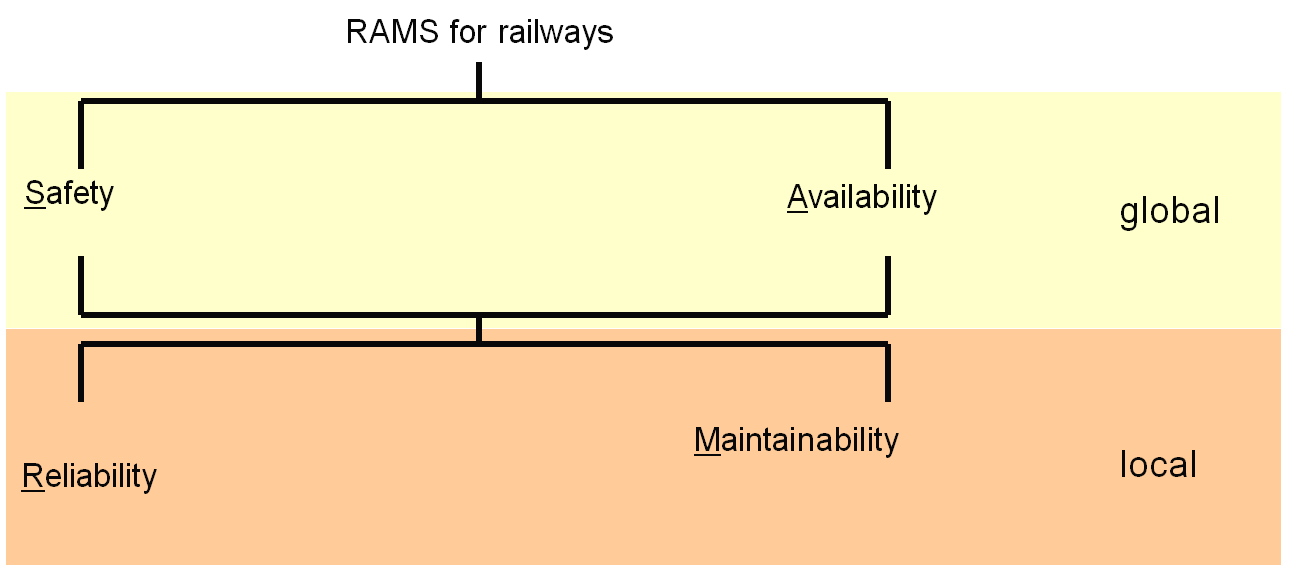
\includegraphics[width=0.7\linewidth]{images/bld_RAMS-Railway-50126}
\caption{RAMS for Railway elements and their relations \cite{Schnieder.2013}}
\label{fig:RAMS-EN50126}
\end{figure}

These depenences between the local and global system charcteristics and the static and dynamic system aspects are shown in figure \ref{fig:Reliability-RAMS}. 

\begin{figure}[htbp]
\centering
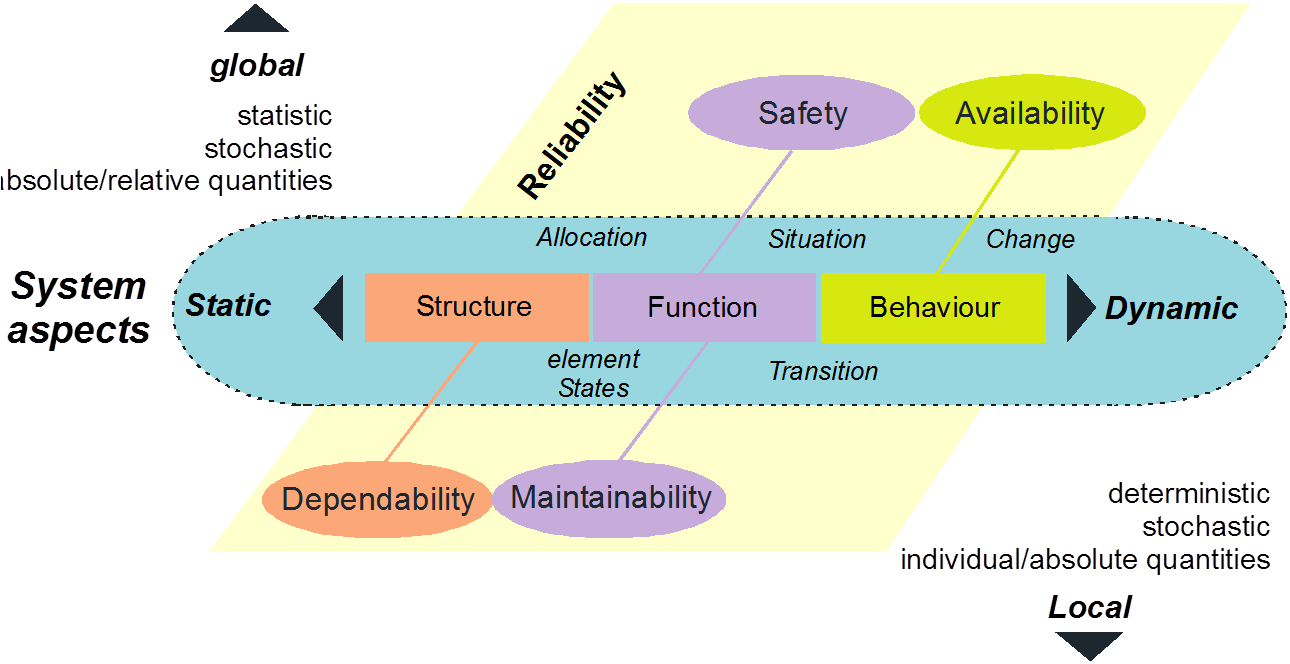
\includegraphics[width=0.7\linewidth]{images/bld_Reliability-system-characteristics}
\caption{Systems Characteristics and their relations to RAMS in Railways \cite{Schnieder.2013}}
\label{fig:Reliability-RAMS}
\end{figure}








\subsection{Probabilistic Safety Concept}

The EN 50128 standard defines safety as the ``freedom from unacceptable levels of risk of harm to people", which shows that the safety approach required by the CENELEC standards is risk-based.

\paragraph{Risk}

 As the risk is defined as the ``combination of the rate of occurrence of accidents and incidents resulting in harm (caused by a hazard) and the degree of severity  of that harm" this approach is based on a probabilistic understanding of event occurrence. The overall relations between all these safety-related terms used to define the safety properties, characteristics and quantities are outlined by the Risk-Genesis-Model of Schnieder, which is shown in the following figure \ref{fig:Risiko-Genese-Modell-eng} \cite{Schnieder.2010}.

\begin{figure}[htbp]
\centering
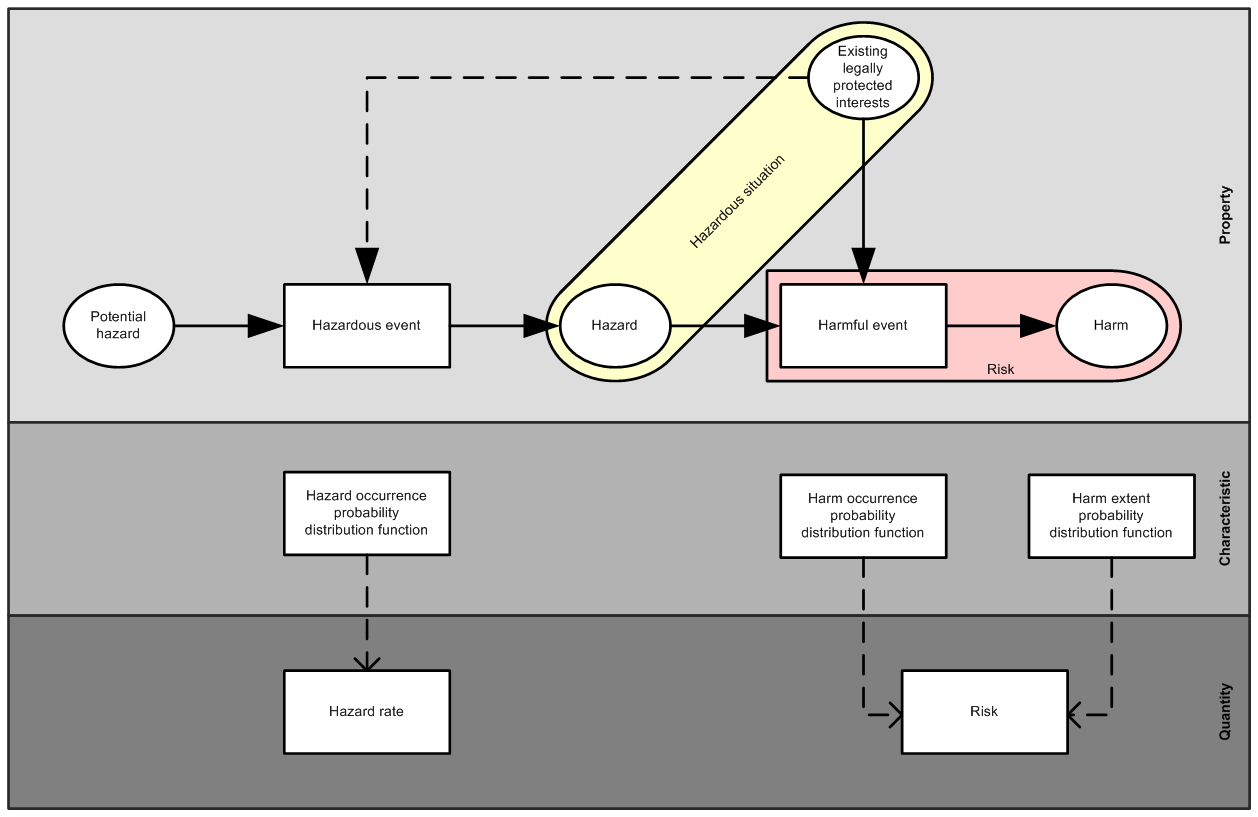
\includegraphics[width=0.8\linewidth]{bld_2013-06-19_Risiko-Genese-Modell-eng-2-0_jw}
\caption{Risk-Genesis-Model showing the relations between the safety-related terms \cite{Schnieder.2010}}
\label{fig:Risiko-Genese-Modell-eng}
\end{figure}

This demonstrates that the first step is to define the system properties, specifically identifying the harms and their related hazardous situations. This has to be performed during a system hazard analysis. Afterwards the respective properties have to be determined by assessing the risk concerning the identified hazards. Based on this work safety integrity levels can be assigned to all system functionalities which are then allocated during the design to certain parts of the operational equipment. As this work is closely related to all design decisions, it has to be done iteratively for all abstraction levels during the system design. 

\begin{figure}[htbp]
\centering
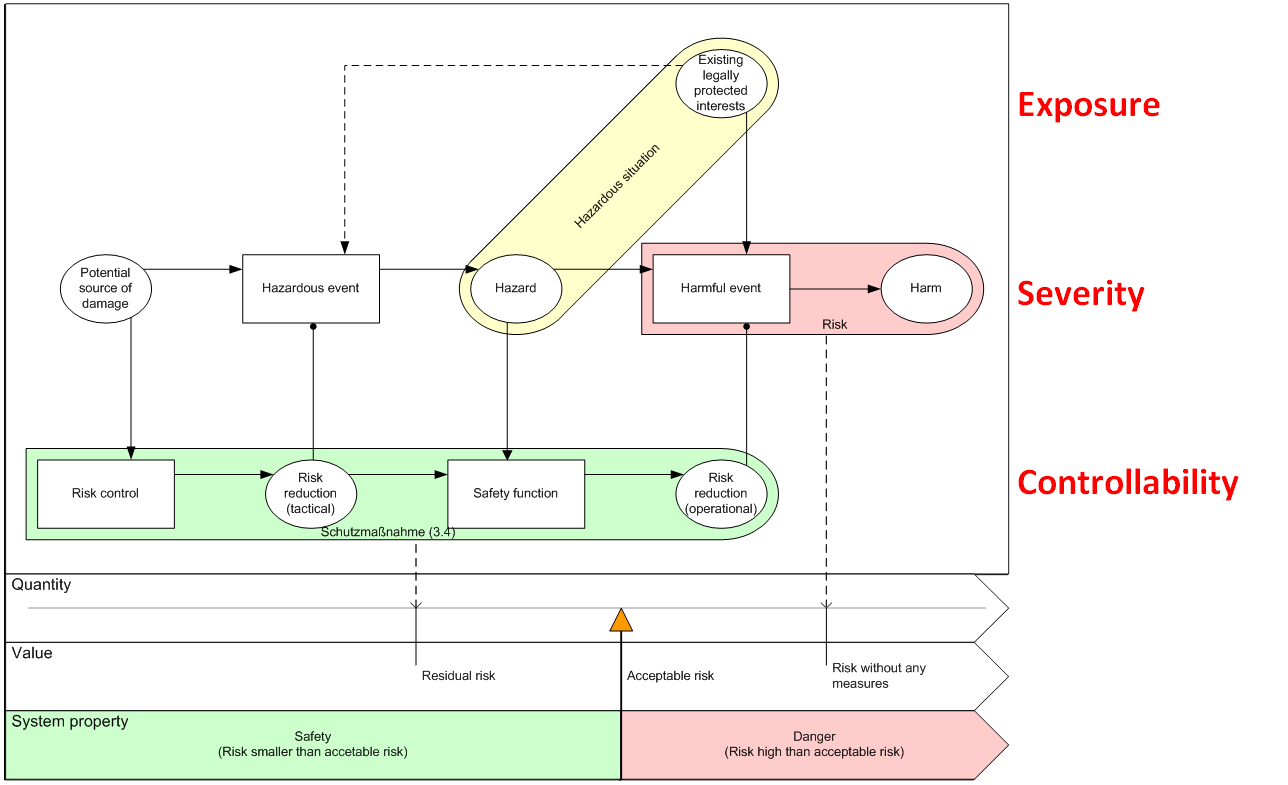
\includegraphics[width=0.9\linewidth]{bld_2013-06-19_Risk-control-modell_1-0_jw}
\caption{Risk control process \cite{Schnieder.2013}}
\label{fig:Risk-control-modell-eng}
\end{figure}

\paragraph{Safety Integrity Level}

The safety integrity level represented the acceptable risk for every part of the system. The risk control process as it is presented in figure \ref{fig:Risk-control-modell-eng} is then performed to ensure that the safety integrity levels are reach by every part of the system.

Since software itself does not fails in the way technical equipment does the specific software safety integrity level represent a qualitative measure with respect to the required degree of correctness for the software functionality than a qualitative value for the likelihood of failing. To reach the needed degree of correctness for the software various design, verification and validation methods are required corresponding to the assigned software safety integrity level. This process leads to safety requirements which have to be implemented in the software design as well as verified and validated. Respectively the EN50126 describes the safety design process as a series of safety tasks for each life cycle phase. This task are related to a number of safety artifacts which are created, used and adapted over time through the different safety design activities.


\subsection{Safety Case}

The EN 50129 states that evidence of quality management, safety management, as well as functional and technical safety have to be provided for safety acceptance. The safety case shall be the structured safety justification document demonstrating that these conditions have been satisfied.
Therefore, the British Ministry of Defence defines a safety case as “a structured argument, supported by a body of evidence that provides a compelling, comprehensible and valid case that a system is safe for a given application in a given environment.”\cite{MinistryofDefence.2007} This definition emphasizes the distinction between the “argumentation” and the “evidences”, which corresponds to the distinction between rules coming from the legal requirements and facts resulting from the actual working process. This clear distinction between the safety argumentation and the evidences helps to structure the safety case and improvement of the discussions with the legal authorities.\cite{Muller.2010}

%\subsection{Safety Glossary}

%\textbf{Added via the glossary documentation process for openETCS}

\chapter{Document Evolution}

This document will be further specified with the progress of the design process to update and detail the corresponding hazard and risk analysis methods. This specifically reference to the refinement of safety properties on different modeling levels and their corresponding verification and validation methods. All resulting changes and additional safety activities have to be maintained according to the EN~50128 and document according to the overall safety case process. 

The openETCS development plan presented in chapter \ref{sec:development-process} is based on the available information in the Quality Assurance Plan and from WP 2 D2.3 and D2.4. As the development methods and processes are still evolving this document has to be adopted accordingly.

Concrete methods to verify and validate safety relevant properties derived from the hazard control methods descriped in this document, will be specified in the Verification and Validation plan. Also the tools used to support those activities will be detailed in this plan.

\chapter{OpenETCS Development process}
\label{sec:development-process}

The main products of the openETCS project will be the OpenETCS specification model used to generate the OpenETCs on-board software and the OpenETCS tools chain development, which is used to formalizes the ERA Specifications for ETCS, generate the Software Code and perform verification and validation activities. Both parts have their own development process, but the focus focus hazard and risk analysis and the safety case shall be on the software development process. The openETCS tool chain shall only be considered with respect to its role in the software development process as the tool qualification is mainly out of this project.
The safety related activities 

\section{Formalization and software development}

The software development in the OpenETCS project shall be performed as an open, model-based, agile Software development. The respective combination of methods used during the development process shall comply with a SIL 4 development process according to EN 50128 for which the requirements are analyzed and shown in detail in D2.2. The overall openETCS Software development process presenting the development principals how the on-board unit requirements for ETCS shall be formalized first in a semi-formal SysML architecture model and afterwards in a detail formal SCADE behavior model, which is the basis for the automatic source code generation, are outlined in WP 2 D2.3 and D2.4. 

The detailed principals and phases of this development process including all related artifacts and used tools have to be presented in the Quality Assurance Plan.  As the project continues this development process and the supporting tools are still evolving, respectively the detailed development description has to be updated in the Quality Assurance Plan continuously.

\begin{figure}[htbp]
\centering
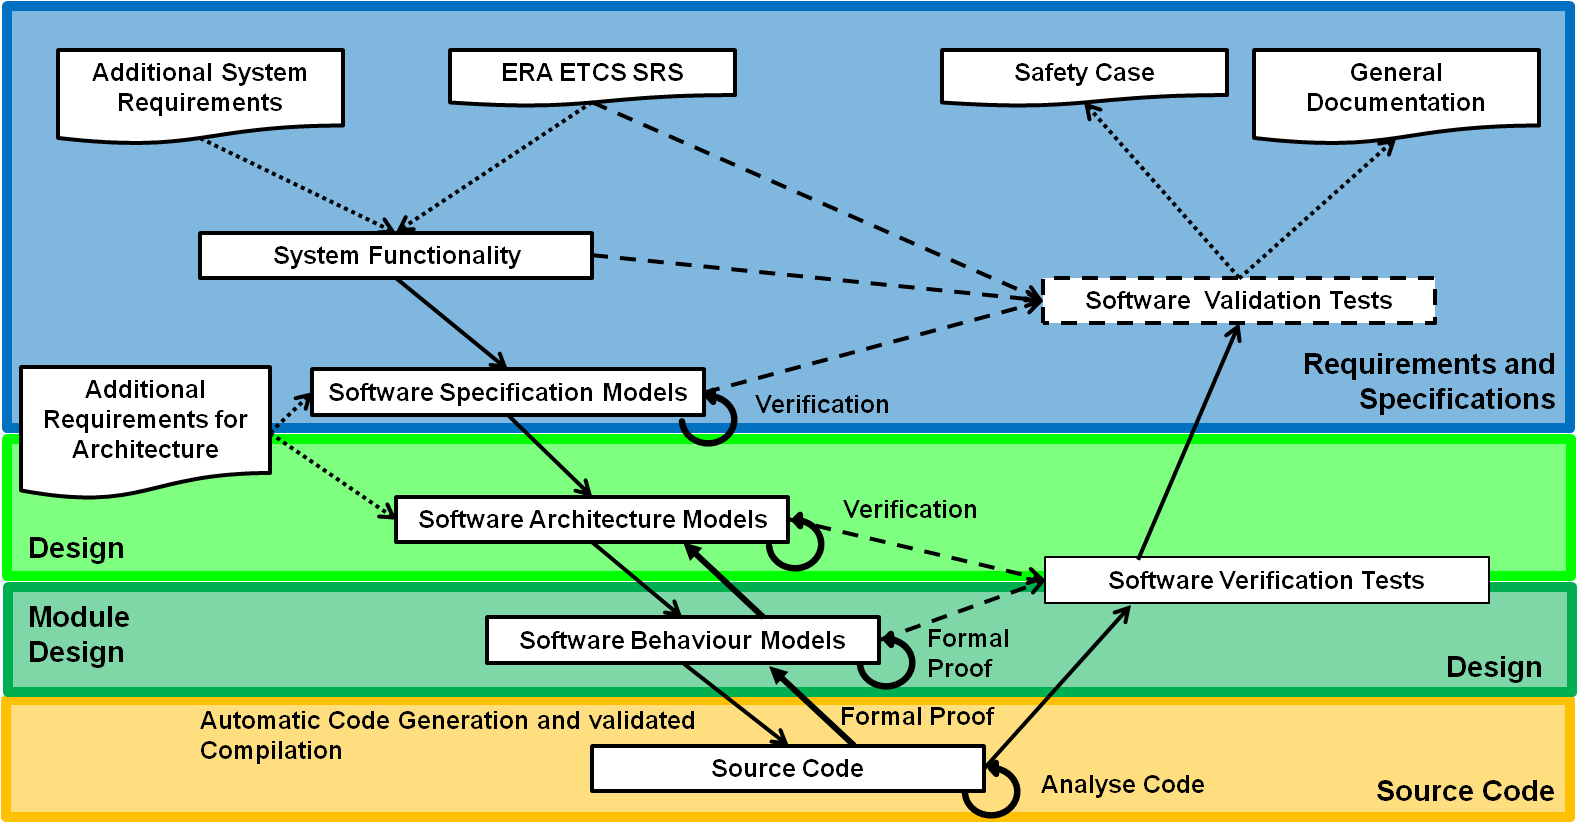
\includegraphics[width=0.9\linewidth]{./images/openETCS-Software-Development}
\caption{Overall openETCS software development process}
\label{fig:DevopmentProcess}
\end{figure}

Figure \ref{fig:DevopmentProcess} shows the general artifacts for the openETCS Software development mapped to the EN 50128 V model development life cycle. As the Verification and Validation activities are specific to the design artifacts further details are not available at this point. The Verification and Validation plan describes a number of methods which can be applied for different properties in the context of the openETCS development principals.

Corresponding to the development artifacts the openETCS development process has 5 main distinguishable phase show in table \ref{tab:DevelopmentPhases}. Every phase besides the validation phase is mostly supported by one means of description and one corresponding tool, but the overall traceability of the development requires linking requirements and design elements between all phases. 

\begin{table}[htbp]
  \centering
  
  \caption{Phases openETCS software development process}
\begin{tabular}{|p{1cm}|p{2cm}|p{7.5cm}|p{2.5cm}|}
\hline \textbf{Phase} & \textbf{Name} & \textbf{Description} & \textbf{Main Tool component} \\ 
\hline P1 & Software Requirement Phase & Requirement input documents converted to a ReqIF format and informally analyses. The analysis specifies relationships between requirements and revises parts of the requirements to obtain a detail and atomic abstraction level usable for moralization. To support thus the requirements are categorized and grouped. & ProR \\ 
\hline P2 & Software Architecture Modeling Phase & Building a SysML based on the informal analysis using the categorization of requirements. The architecture model focuses on functional blocks and data flows. & SysML Papyrus \\ 
\hline P3 & Software Behavior Modeling Phase & Building the SCADE model for the separated basic functional blocks. The SCADE model describes the detailed behavior for the function using the data flows. & SCADE Suite \\ 
\hline P4 & Code Generation Phase & Based on the SCADE Behavior Model C code will be automatically generated. This C code is than compiled to executable code which runs on the EVC. & SCADE Suite + C Code compiler\\
\hline P5 & Formal Validation phase & Using test models and model checking techniques, to validate the correct model behavior.  & Various tools \\ 
\hline 
\end{tabular} 
\label{tab:DevelopmentPhases}
\end{table}

Although the phase represent different working steps in the life cycle according to EN 50128 the agile development process applied in openETCS induces that the phases are performed iterative during the development process. Respectively, the traceability linking in combination with the verification methods has to ensure that changes in one phase of the development are adopted for all linked artifacts up- and downwards in the development process.

\section{Interfaces to Safety Activities}

As safety is a system property the software development has to be performed according to the safety functionalities allocated to the software. Thereby, the resulting Software SIL defines the combination of quality methods to be performed to ensure that all requirements including the allocated system safety requirements are implemented correctly. To provide all needed justification that the required Software SIL is reached, the development has provide complete documentation for the safety case. As the openETCS software development is not part of a specific system development, but has the objective to specify and implement the overall ETCS functionality, it has to interact with a respective generic safety management process and take the overall safety requirements for a train control system into account. As show in figure \ref{fig:SafetyProcess} the over all development is determined by a number of interactions between design, verification and validation and the general quality and safety management.

\begin{figure}[htbp]
\centering
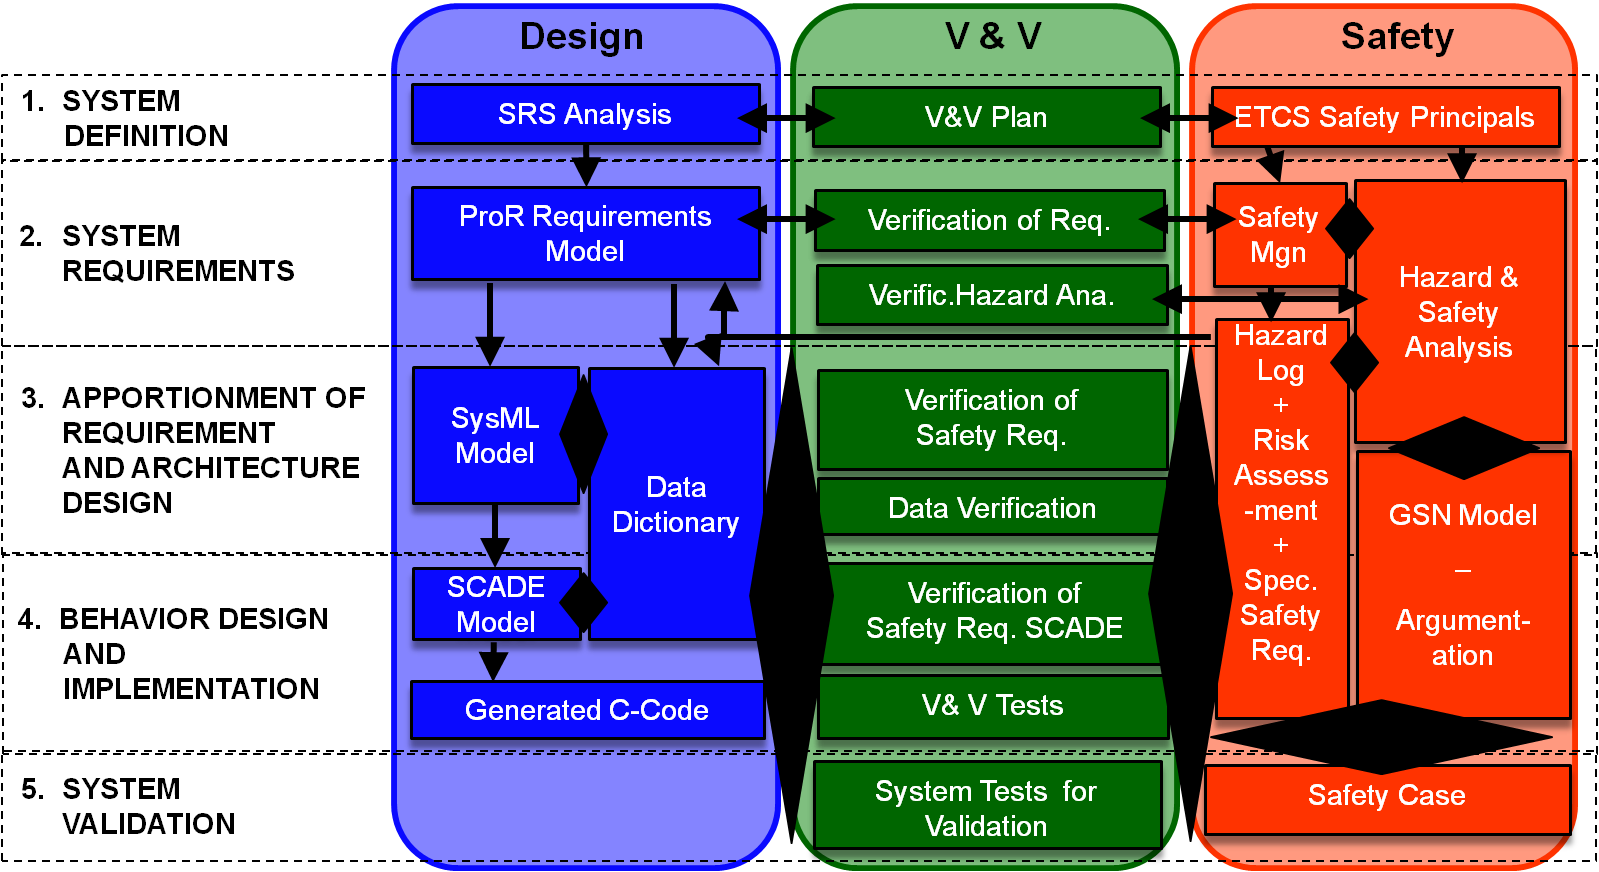
\includegraphics[width=1\linewidth]{./images/openETCS-Software-Safety-Development}
\caption{OpenETCS development relations between design, verification and validation and safety activities}
\label{fig:SafetyProcess}
\end{figure}


\subsection{Interface to Quality and Safety Management}

In parallel to the design process the safety management process has to perform hazard and risk analysis methods for the software design to ensure that the design concept can reach the expected safety integrity level for the overall system. Thereby, potential hazards resulting from the software functionality and its design have to be identified and their risk has to be assess in the system context. To control the risk respective measures have to be taken, which be realized through additional safety requirements to which the design has to be conform. The hazard log represents the central element of this safety management as it collects the hazards and manages the respective risk control.

As the Software SIL determines the development methods which have to be applied to ensure a correct development, the quality management has to ensure that these methods are chosen according to the standard and are applied correctly. This has to be specified in the Quality Assurance Plan and to be documented in the overall safety case. 

\subsection{Specific Interfaces to the Design Process}

To be able to respect the system safety requirement these have to be apportioned to the different software components. This has to be done for all abstraction levels during the during the system design. 

\subsection{Interface to Verification and Validation}

The verification activities have to ensure that all system safety requirements have been apportioned and implemented correctly at the respective software component.

The validation activities have to ensure that the overall software implementation matches the actual requirements. Therefore, it has to be ensured specifically that the Software in it system context respects the overall system safety requirements.

The verification and validation plan do specify the appropriate methods used. The verification and validation reports as evidence for the qualified software development become part of the safety case.


\chapter{Hazard and Risk Analysis}
\label{sec:hazardandrisk}
The safety design process and the resulting documentation constitute the main documents for the system approval, as it is required by European and national law to do everything reasonable expectable to prevent harm. Accordingly the CENELEC standards build the common technical rules for the development process. The Common Safety Methods present a concept based on the EN50126 how the risk evaluation and management has to be performed. 

Therefore the main references concerning the safety design process are the CENELEC standards, mainly the EN50126 on how the safety aspects have to be handled as part of the RAMS management over the development process. The overall risk evaluation concept is also defined at this point. The specific concerning the safety case preparations are defined in the EN50129 including the Safety Integrity Level concept. 

Since the ETCS system specification for the on-board unit shall be formalized and implemented in the software during the openETCS software development, the specific safety requirements for the on-board unit have to been determined according to the overall system requirements. These are mainly given by the following two parts of the CCS TSI:

\begin{itemize}
\item UNISIG SUBSET-026	System Requirements Specification 	(Version 3.3.0)
\item UNISIG SUBSET-091 Safety Requirements for the Technical Interoperability of ETCS in Levels 1 and 2 	(Version 3.2.0)
\end{itemize}

In relation to SUBSET-91 further documents should be take into account to derive specify safety aspect:

\begin{itemize}
\item Part of TSI Annex A
	\begin{itemize}
	\item SUBSET-036
	\item SUBSET-037
	\item SUBSET-040
	\item SUBSET-041
	\item SUBSET-098
	\end{itemize}
	
\item Not part of TSI Annex A
	\begin{itemize}
	\item SUBSET-039
	\item SUBSET-078
	\item SUBSET-079
	\item SUBSET-080
	\item SUBSET-081
	\item SUBSET-088
	\end{itemize}
\end{itemize}

Based on these overall safety goals as specific hazard and risk analysis for the software subsystem has to be performed to allocate the requirements and set-up the openETCS hazard log as shown in figure \ref{fig:SafetyProcess}. Cased on the principal software architecture the risk can be assess, which then leads to the definition of risk control measures. These are the basis for specific safety requirements for the on-board unit software design and its verification and validation. During the development these requirements are adopted if necessary for the different abstraction levels from the high level model down to the source code. The safety case, which shall be supported by a Goal Structured Notation (GSN) \cite{GSNwebsite} model as presented in chapter \ref{sec:safetycase} has to present all needed documentation to show that these leads to the required risk level.

\section{General ETCS Safety Principals}

Based on the ETCS reference architecture Subset 91 gives the role of ETCS as train protection as the following:

\begin{center}
\textbf{"To provide the Driver with information to allow  him to drive the train safely and to enforce respect of this information, to the extent advised to ETCS."}
\end{center}

Respectively, the Core Hazard for the ETCS reference architecture is defined as the following in Subset 91:
\begin{center}
\textbf{"Exceedance of the safe speed or distance as advised to ETCS."}
\end{center}

Based on the role of ETCS and its respective SIL 4 quantification the maximum allowed rate of occurrence (Tolerable hazard rate) of the ETCS Core Hazard for ETCS on-board is
\[1.0\times10^{-9} hour^{-1} train^{-1}.\]
The same value is specified for the corresponding track-side.

Adapted form the ETCS system safety analysis presented in Subset 88 the Annex A of Subset 91 presents the List of Hazardous Events inside ETCS that might cause the ETCS Core Hazard to occur, either alone or in combination with other failures. These are the events not eliminated by the operational analysis. 34 of these hazardous events are allocated to the Kernel, which make them the basis for the on-board software hazard and risk analysis. 


\section{Proof of concept}
\label{sec:Proofofconcept}

To evaluate the hazard and risk analysis process in the openETCS development environment a proof of concept has been performed during the VnV Level 1 activities in WP 4 by project partners Systerel, All4Tec and AEbt. As the respective design artifact for the proof of concept a SysML modeled formalizing one part of Subset 26 has been chosen: 

\begin{center}
\textbf{"\S 3.5 Management of Radio Communication (MoRC)."}
\end{center}

This model has been created by the project partner Siemens during the design process first in SCADE and then extended to a SysML model. The Model can be found under \url{https://github.com/openETCS/model-evaluation/tree/master/model/SCADE_Siemens/MoRC_System/MoRC_System/SysML_Model}. For the Proof of Concept only the SysML model has been used as the scope was on the hazard and risk analysis for the SysML architecture allocation.

To do so the following hazardous event given in Subset 91 has been identified as the event mainly related to this part of the specification:
\begin{center}
\textbf{“KERNEL-6 Manage communication session failure” which results an “RADIO (INFILL) Transmission data consistency failure (safety related transmission function)”.}
\end{center}

The following task have been performed during the Proof of Concept as examples for the activities during a hazard and risk analysis. 
 
 
\begin{enumerate}
\item Conformity comparison for the MoRC
	\begin{itemize}
	\item Conformity comparison regarding sub functions between Subset 26 and SysML model
	\item Conformity comparison regarding Input and Output data between Subset 26 and SysML model
	\end{itemize}
	
\item Safety Analysis for the MoRC
	\begin{itemize}
	\item Hazard \& Risk analysis for each sub functions
	\item Derivation of safety Target (SIL) for each sub functions
	\item Derivation of safety requirements for each sub functions
	\end{itemize}
	
\item Safety Assessment for the MoRC
	\begin{itemize}
	\item Derivation of the safety requirements
	\item Assessment of the model against these safety requirements
	\end{itemize}
\end{enumerate} 
 

The first task conformity comparison has been performed to verify the model, as no formal verification process has already been performed on the chosen preliminary model. The conformity was passed, as all sub function of the subset 026 function (MoRC) and those of the model match together and all Input \& Output data for each sub function of the subset 026 function and those of the model also match together. 

 
The second task Safety Analysis was performed using methods for three different safety activities as defined in the EN 50129 standard: hazard identification,
risk estimation and evaluation, derivation of the Safety requirements. In general hazard identification and risk analysis are performed using traditional approaches like FMECA or HAZOP. In the case of openETCS since models are available a model-based, computer supported approach (based on the Tool “Safety Architect” from the company ALL4TEC) for hazard identification has been used in addition.
Both results have been compared at the end to validate the results.
 
For functions coming from the Subset 026 a hazard and rick analysis has been already performed, including a SIL allocation as presented in Subset 091. All these functions have a SIL 4 safety requirement; therefore sub function from these functions shall have also a SIL 4 safety requirement. For functions and corresponding sub function coming from others sources than the Subset 26 a SIL allocation on the basis of techniques described in the standards EN 50126, 50129 or IEC 61508-5 shall be performed.
 
The third Task of the process consists in performing a Safety Assessment, which implies derivation of safety requirements and the following assessment of the model against these safety requirements. The derivation of the Safety requirements required knowledge in the function being analyzed, the interfaced components, the ETCS in general and CENELEC standard.
 
 
The details results for the Proof of Concept can be found at \url{https://github.com/openETCS/validation/tree/master/VnVUserStories/VnVUserStoryAll4Tec-AEbt}. 

Overall the Proof of Concept has confirmed the correctness of the model as far as this has been possible in the limited scope. 

The FMEA has identified 23 hazardous events in the subsystem which could lead to the Kernel 6 event. As measure to prevent this occurrence of these events 18 safety criteria have been derived.  

The model-based safety analysis showed 12 safety assumptions related to over 40 granular function events. These are related to the assumed unwanted behavior in different subfunction blocks. Overall both methods seam to create comparable results, but due to the status of the model and the complexity of the mathematical model-based analysis both results are difficult to match. Respectively, the model-based analysis has to be specified further to fit the modeling process. But due to the size of Subset 26 on-board function, the model-based analysis is in the focus to lower the amount of manual work.
 
As the proof of concept has clear shown that the process is able to derive Safety requirements, which can be allocated to different specification based on the software architecture, the results can be used to define the openETCS hazard and risk analysis process.
 
\section{Hazard and risk analysis supporting tools}

Supporting software tools are needed to handle the safety artifacts and to some degree to more efficiently perform the safety design activities. As some safety artifacts like the safety requirement specifications and the safety backlogs are closely related to design artifacts the same tools can be used. Especially all requirements should be handled by one tool to ensure full traceability and provide one main interface for the verification and validation activities.

Depending on the methods used for hazard and risk analysis appropriate tools are needed to perform the analysis, collect the hazards and associated risks in the hazard log and to evaluated possible risk control measures. Thereby, traceability has to be guaranteed between all activities. As the main architecture will be designed in SysML, safety analysis tools like the Safety Architect Tool will be used to analyze the hazard propagation in the functional decomposition and to derive the resulting risk level. In this way short feedback iterations to the design process can be realized.

\chapter{OpenETCS Safety Case}
\label{sec:safetycase}

In general the safety case has to present to the assessing authority that the development has be done according to the required standards and that the product confirms to the quality and safety level corresponding to the aspired utilization. 
To do so the present chain of argumentation has to state the requirements for the product development, its derived specifications and the evidence that the work has been done accordingly. To do this the safety case has to collect and combine documents from many different activities during the work process. As these documents are usually produced and stored in different places and formats studies have shown that a large amount of time to produce the safety case is spent on searching for document, maintaining document contents and maintaining document references \cite{Muller.2010}. 

\section{Structure}

As the openETCS development has the objective to produce a reference formalization and implementation for the ETCS on-board unit, which can be used by interested parties during further development, it is highly important to collect all relevant documents in a way, that the can directly be used even for safety relevant system development. If thereby the distinction between basic assumptions, safety argumentation and evidences for the openETCS development is presented properly in the safety case the discussions with the legal authorities is improved and reusability is made easier. 

Overall the openETCS will separate between the following three kind of evidence in compliance to the safety acceptance conditions stated in the EN 50129. 

\subsection{Quality Management Evidence}

Since the openETCS project as a research does not have the objective to conduct all steps needed for a vital on-board unit development, the resulting safety case will be generic in many parts only giving the requirements and basic safety strategies, but lacking the actual evidence. However, the overall safety argumentation has to be set up to meet SIL 4 requirements. Therefore the safety case has to show that the methods chosen in the openETCS development process satisfy the EN 50128 quality requirements and which documents have to be created during the process to obtain the required evidence. Basis for this work will be the Quality Assurance Plan, which builds the basis for all quality management activities.

\subsection{Safety Management Evidence}

As detailed in chapter \ref{sec:hazardandrisk} the overall safety argumentation has to demonstrate that during the development process the higher-level safety requirements have been addressed and that accordingly the on-board software satisfies the safety level. As this will be done using the basic process presented in chapter \ref{sec:hazardandrisk}, the safety case has to specify the traces from high-level hazardous events to all subsystem requirements allocated to the openETCS software architecture and their verification and validation. Therefore, the safety case has to present evidence that the chosen methods are sufficient to demonstrate compliance to the requirements and that they are applied in a consistent process which ensures that all safety requirements are respected and validated.


\subsection{Functional and Technical Safety Evidence}

The main evidence for this part will be the validation results which proof that the actual models and/or the code satisfies the overall safety principals. For all evidence to been produced during the openETCS process the safety case clear has to show the specific artifacts need to enable every adapter to provide these evidence later while reusing already provided evidence in the context of the overall safety argumentation.

\section{Model-based Argumentation}

The openETCS safety case shall present a transparent and easy to understand argumentation chain referring to the relations between the sequential and parallel processes in the development process and the respective requirements in the normative EN 50129 safety case. Capitalize on the basic principals applied during the openETCS development the safety chase can be enhance by using a model-based representation connected to the central data base to reference the respected artifacts \cite{Muller.2010}. Thereby, the model provides a graphical representation of the argumentation chain, which makes it possible to directly identify in which development step which requirements is address and which are the respective artifacts containing the design and the corresponding evidence. 

In this way the generic safety case present the over argumentation structure connecting requirements, design artifacts and evidence. The specific openETCS safety case is then provided trough the linking to the github data based providing document versions and status information to ensure consistence throughout the evolving documentation.

\subsection{Goal Structured Notation}

Interviews performed during the INESS project have shown that graphical argumentation structures ease the discussions between with legal authorities as it provides a look on the essence of the argumentation strategy in an easy way. During the method evaluation the Goal Structuring Notation (GSN) \cite{Kelly.2004thegoal, GSNwebsite} has been identified as suitable argumentation notation, already use in industrial projects, to  graphically  to model the relations between individual requirements, methods and evidence in a safety case. The argumentation demonstrates how each requirement will be address by a tree structure of derived subgoals and the resulting evidence to satisfy these goals as shown in figure \ref{fig:GSN-SafetyCase}. The different notes in the tree will be linked to the openETCS development artifacts in the github document management system. Additionally the artifacts will be linked to the modeled documentation of the EN 50128 development process during the corresponding phases to demonstrate the process conformity. 
 
\begin{figure}[htbp]
\centering
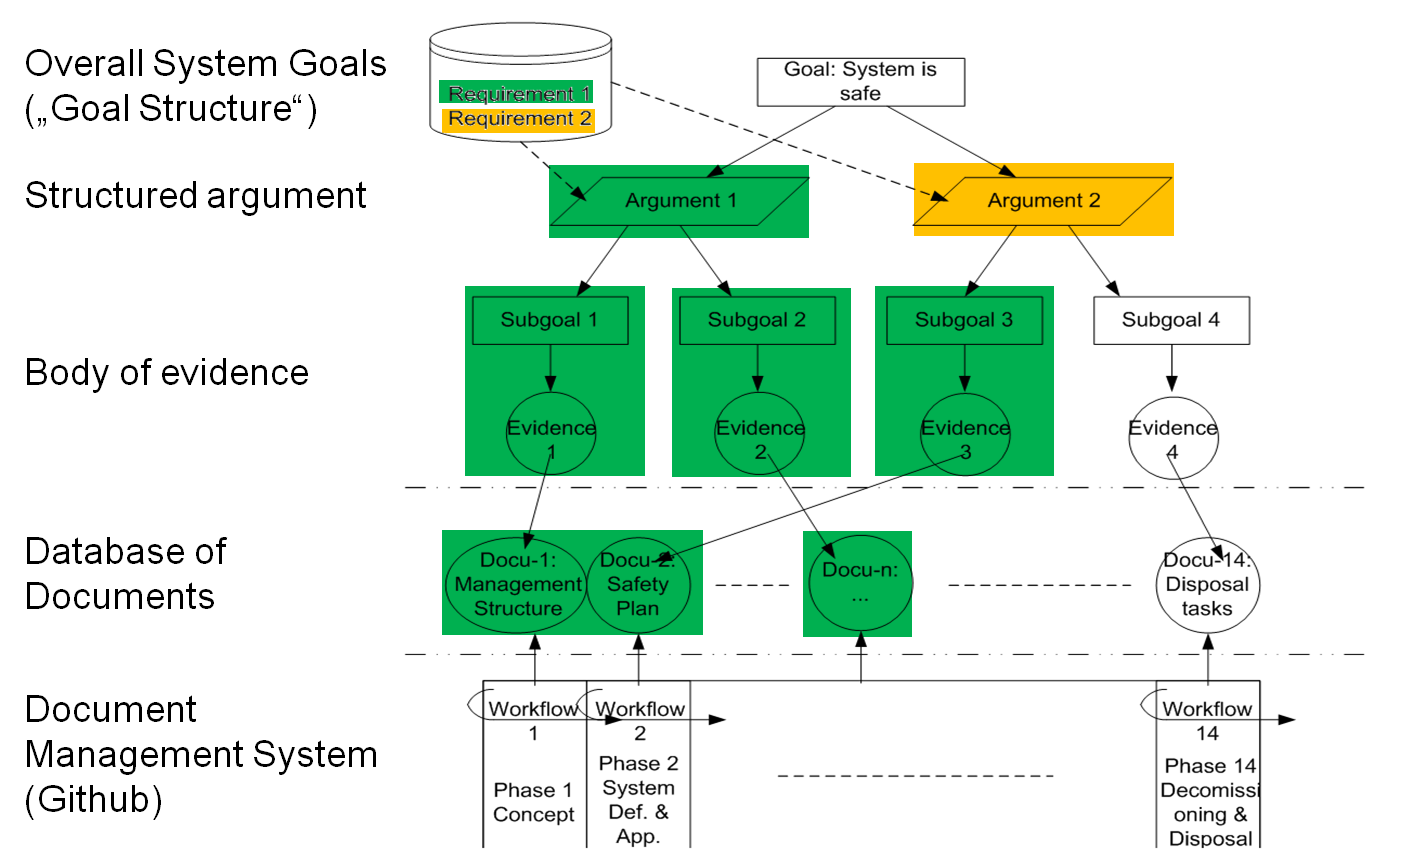
\includegraphics[width=0.9\linewidth]{./images/Structure-SC-GSN}
\caption{Structure model-based safety case using GSN}
\label{fig:GSN-SafetyCase}
\end{figure}

 In addition, the graphical model and its reference to the different artifacts provides as valuable option for external and internal parties to locate and retrieve the right information from the diverse data base structure of the opneETCS project.

\subsection{Safety case supporting tools}

To support the proposed model-based safety case a safety case editor to model GSN argumentation structures is needed. For the artifact relations the editor has to provide an interface to connect individual model element to specific artifacts in the document management system. An ideal support for the automatic evolution of the safety case would be provide when the interface allows the exchange of meta data concerning the artifacts like status and version, which can be presented in the model to demonstrate the current status.

Since the openETCS development uses the eclipse tool platform and the github document management system as the backbones for the tool integration and the artifact management, the tool supporting this model-based safety case approach shall be able to interact with these two. 

The Assurance Case Editor (ACedit) \cite{aceditwebsite} is a tool implementation of GSN \cite{GSNwebsite} and the OMG  Argumentation  Metamodel  (ARM) \cite{ARMwebsite} to graphically construct argumentation structures to which this tool refers as assurance cases. In addition the tool supports a number of model management techniques including model checking methods that apply to GSN and ARM. As ACedit is eclipse based the evaluation done during the verification and validation level one has determined this tool as the most promising GSN editor. Since the eclipse framework provides an interface to github via the EGit plug-in the document management system integration shall be realized through the eclipse model base.

The GSN editor developed during the INESS project has been dismissed as it is only java based. The effort needed to connect this tool to eclipse and github during the openETCS projet was sat as to high. 
 
\chapter{Conclusion}
\label{(sec:conclusion)}

This document has presents the basic concept for the main safety related activities in the openETCS development as they have been determined during the first verification and validation iteration level of WP 4. As these have been set in respect to a still evolving development methodology and tool chain, the overall process as to be detailed and adopted as the project continues. 

As the openETCS development presented in chapter \ref{sec:development-process} formalizes the Subset 26 requirements using SysML and later SCADE models, the hazard and risk analysis methodology applied at the openETCS development has to be able to allocate all hazardous events relevant for the kernel of the on-board unit to subsystems of the openETCS software architecture. Based on this allocation the resulting risk will be determined leading to safety requirements to control the overall system risk allowed level. 

The results for the proof of this concept conducted during the first verification and validation level by Systerel, All4Tec and AEbt using the benchmark SysML model for Management of Radio Communication and one allocated hazardous event has show that the proposed methodology for hazard and risk analysis provides sufficient safety requirements for the design process. Further specification of the methodology has to be done to support or even replace the manual FMEA or HAZOP with an automatic analysis of the SysML model by the Safety Architect tool. However, the proof of concept has demonstrated that this could be sufficient and the best option to work in short design iterations as the openETCS project plans to do. 

In general the verification and validation activities have to ensure that the safety principal apportioned to the on-board functionality are satisfied. Hence, the main objective for the openETCS safety case as presented in chapter \ref{sec:safetycase} is to provide the fundamental quality and safety principals for the openETCS development as these have to be completed by adopters of the openETCS results for their assessment. Therefore, the general safety argumentation and the concrete evidences shall be clear distinguished to ease applicability and support discussions with different legal authorities.

Modeling the generic argumentation structure and connecting the individual elements to the respective artifacts created during the openETCS development has been identified during the first level iteration as a promising approach to show the relations between requirements, safety strategy and provides evidence. A GSN model combined with direct links to the actual artifacts in the document management system should also help the internal and external discussions concerning the safety strategy. To efficiently use this approach for the safety case preparation the  chosen Acedit editor for GSN has to be interfaced with the github document management system. 

Overall the main methodology for the hazard and risk analysis as well as the safety case work has been defined during the first level iteration but these concepts have to be further refined over the next iterations with the evolving development process.

\bibliographystyle{unsrt}
\bibliography{./ref/ref-HaRA}


%===================================================
%Do NOT change anything below this line

\end{document}


